\documentclass[12pt,oneside,letterpaper]{article}
\usepackage[T1]{fontenc}
\usepackage[utf8]{inputenc}
\usepackage[margin=2.25cm,headheight=26pt,includeheadfoot]{geometry}
\usepackage[french]{babel}
\usepackage{listings}
\usepackage{color}
\usepackage{titlesec}
\usepackage{titling}
\usepackage[framed, numbered]{matlab-prettifier}
\usepackage{changepage}
\usepackage{amsmath}
\usepackage{hyperref}
\usepackage{enumitem}
\usepackage{graphicx}
\usepackage{fancyhdr}
\usepackage{lastpage}
\usepackage{caption}
\usepackage{tocloft}
\usepackage{setspace}
\usepackage{multirow}
\usepackage{titling}
\usepackage{float}
\usepackage{comment}
\usepackage{booktabs}
\usepackage{indentfirst}
\usepackage{lscape}
\usepackage{booktabs,caption}
\usepackage[flushleft]{threeparttable}
% \usepackage[french]{nomencl}
\usepackage{xcolor}
\usepackage{lipsum}
\usepackage{datetime2}
\usepackage{verbatim}

% --- set footer and header ---
\pagestyle{fancy}
\fancyhf{}

\setlength{\parindent}{2em}
\title{} % to reference as \title, dont use \maketitle
\makeatletter\let\Title\@title\makeatother



\lstset{language=Matlab,
style=Matlab-editor,
basicstyle=\normalsize\mlttfamily,
numbers=left,
numberstyle={\scriptsize\color{black}},	% size of the numbers
numbersep=0.5cm											
}

\newlist{steps}{enumerate}{1}
\setlist[steps, 1]{leftmargin=1.5cm,label = Step \arabic*:}
\renewcommand{\headrulewidth}{1pt}
\renewcommand{\footrulewidth}{1pt}
\renewcommand{\rmdefault}{ptm}

%\lhead{\Title}
\rhead{\nouppercase{\rightmark}}
\lhead{\Title}
\rfoot{
\includegraphics[height=0.5cm]{saclay_logo_small.png}} % right header logo
\setlength\headheight{16pt}
\setlength{\footskip}{50pt}
\lhead{\Title} %rightH title
\cfoot{\thepage}

% --- End of page settings ---



\begin{document}
\pagenumbering{roman} 
\begin{titlepage}
\begin{center}
\vspace{2cm}
%\textsc{Oregon State University}\\[1.5cm]

\includegraphics[width=0.4\textwidth]{saclay_sciences.png}~\\[1cm]
\vspace{2cm}

% Title
\hrule
\vspace{.5cm}
{ \huge \bfseries Introduction to the functional programming\\project report} % title of the report
\vspace{.5cm}

\hrule
\vspace{1.5cm}

\textsc{\textbf{Authors}}\\
\vspace{.5cm}
\centering

% add your name here
Yehor KOROTENKO - yehor.korotenko@etu-upsaclay.fr\\
Ivan KHARKOV - ivan.kharkov@etu-upsaclay.fr\\

\vspace{4cm}

\centering \today % see latexmkrc for time zone change
\end{center}
\end{titlepage}


\newpage
\doublespacing
%\addcontentsline{toc}{section}{Table of Contents}
\renewcommand{\baselinestretch}{1}\normalsize
\tableofcontents
\renewcommand{\baselinestretch}{1}\normalsize
%\singlespacing
\thispagestyle{fancy} % force page style

\newpage
\pagenumbering{arabic} 
\fancyfoot[C]{Page \thepage}

\section{Introduction}
Le joueur débute sa progression dans un environnement désertique, à proximité d'une pyramide. Non loin de là se trouve un monument de taille modeste consacré au dieu égyptien Anubis. Une entrée secrète est discrètement située à droite du monument.

\begin{figure}[H]
    \centering
    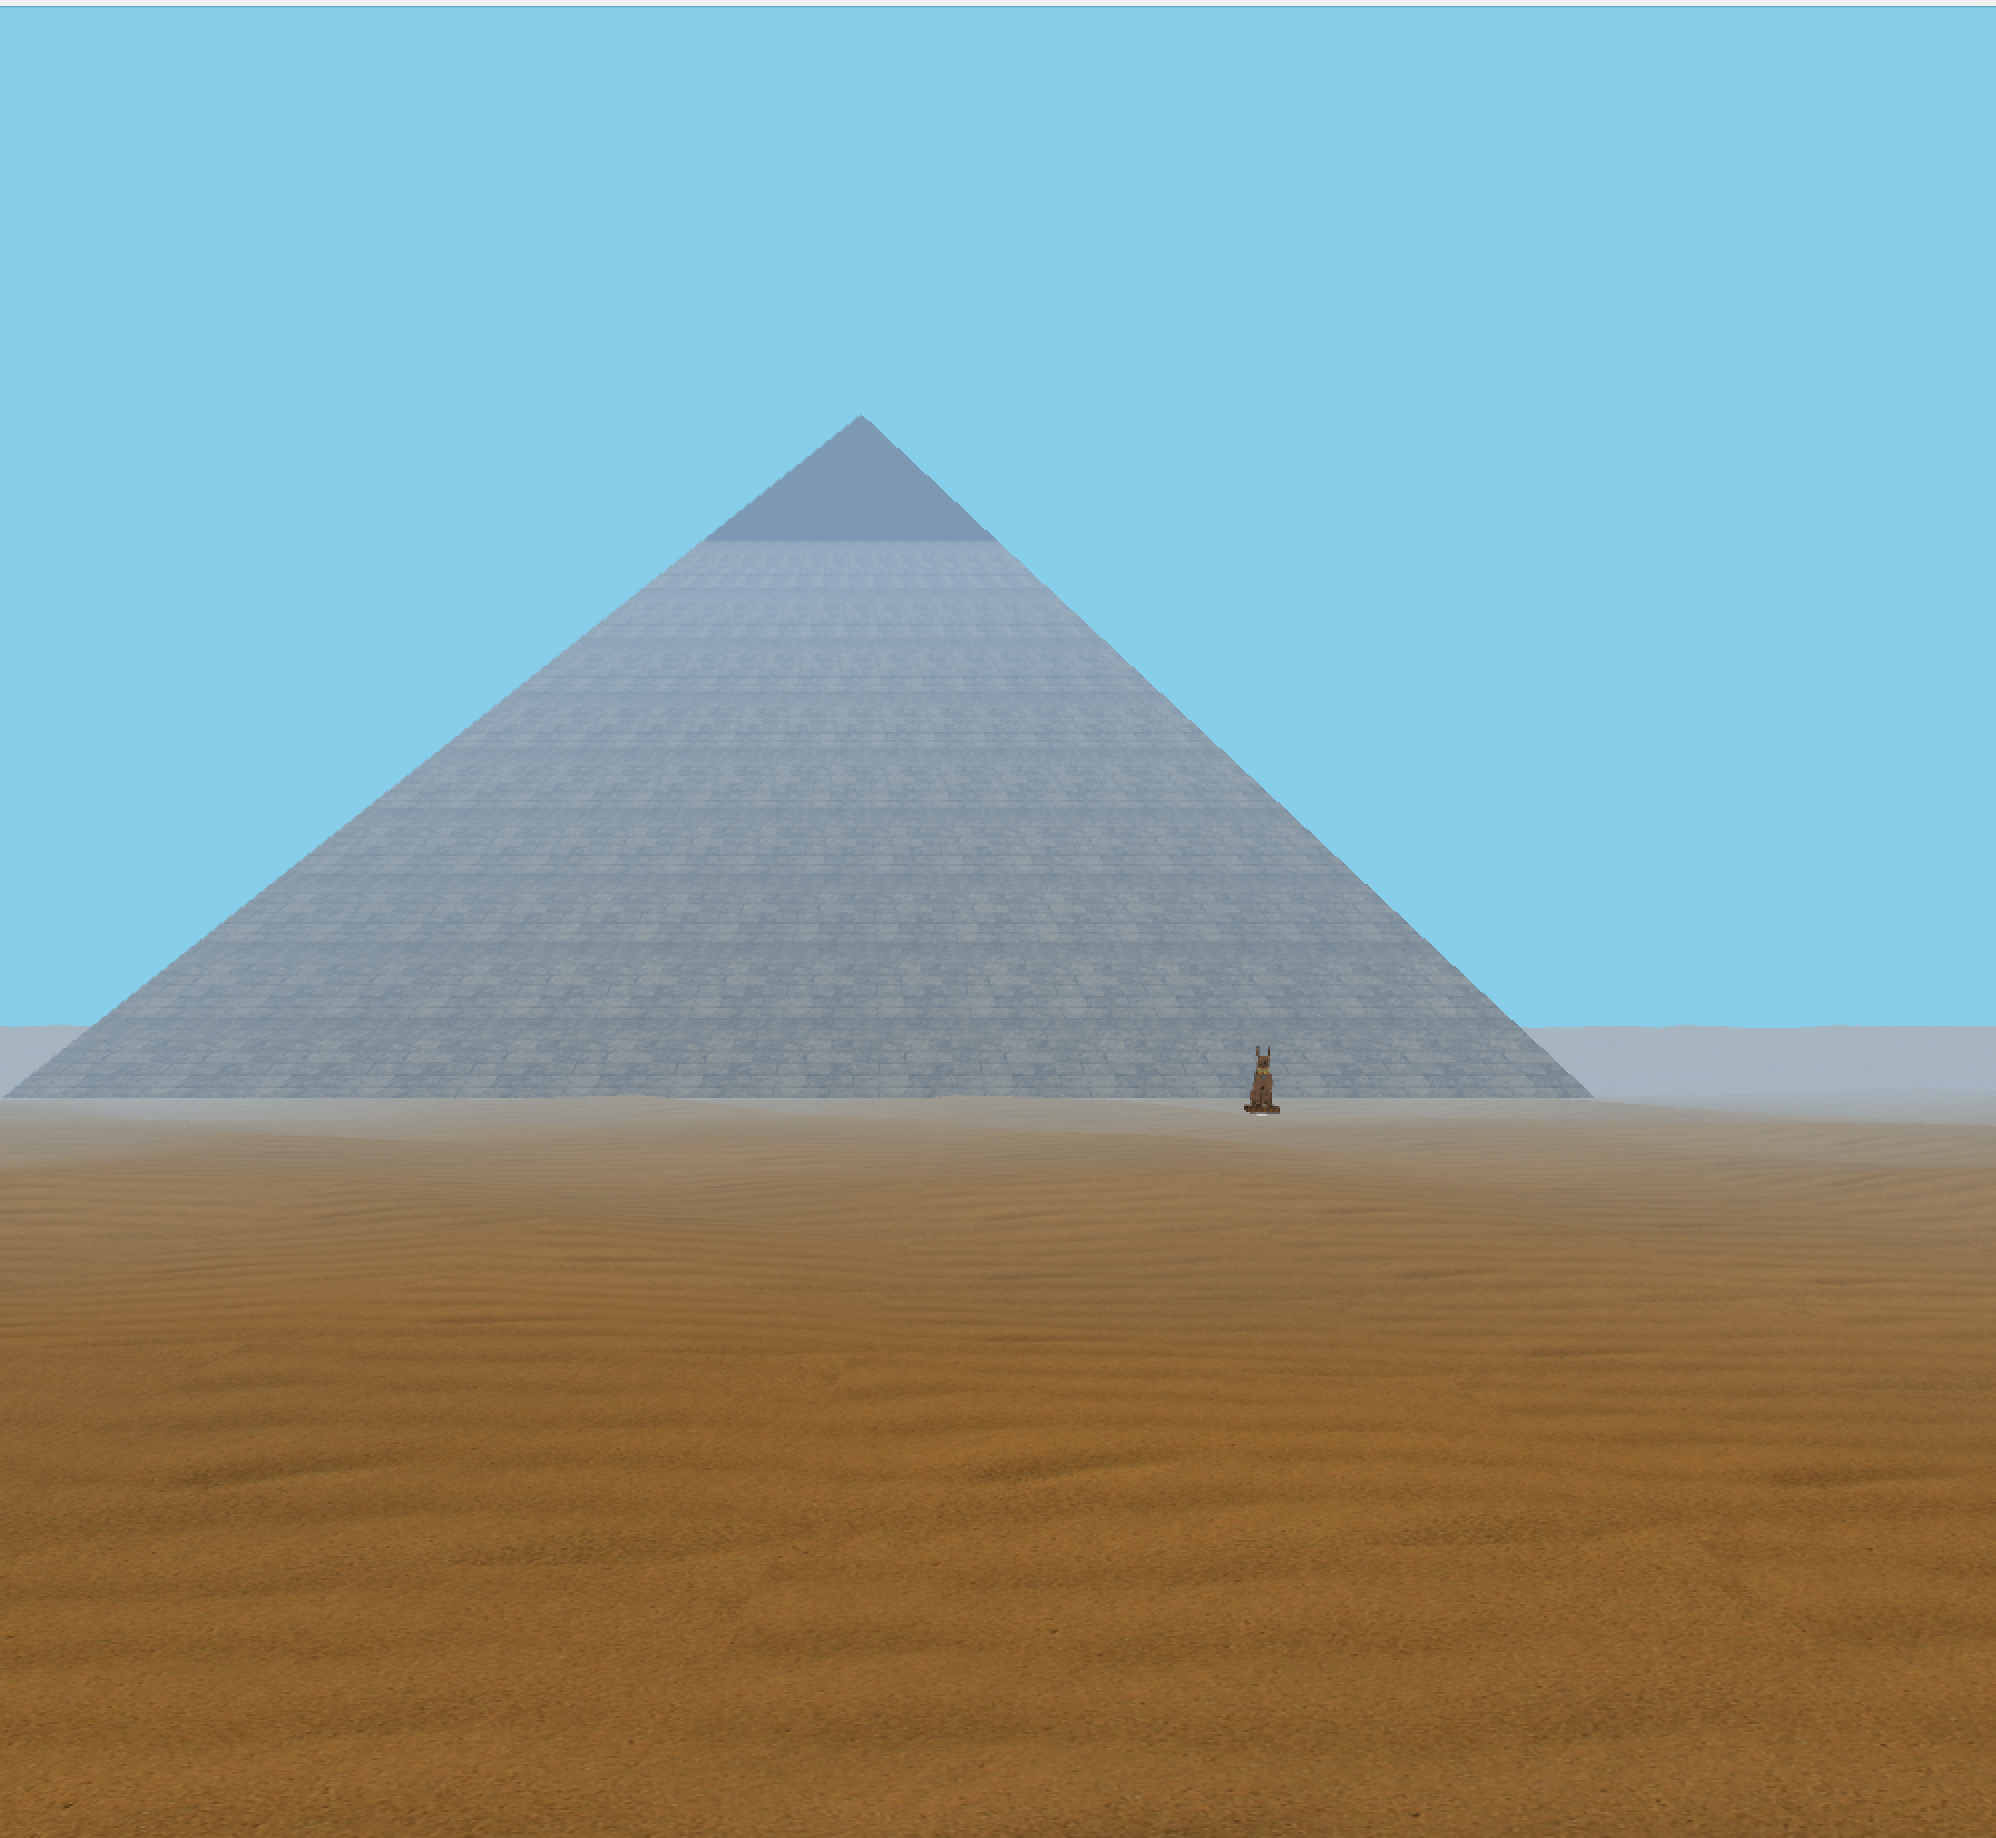
\includegraphics[width=0.8\textwidth]{figures/pyrdamid-big.png}
    \caption{World overview}
\end{figure}

\begin{figure}[H]
    \centering
    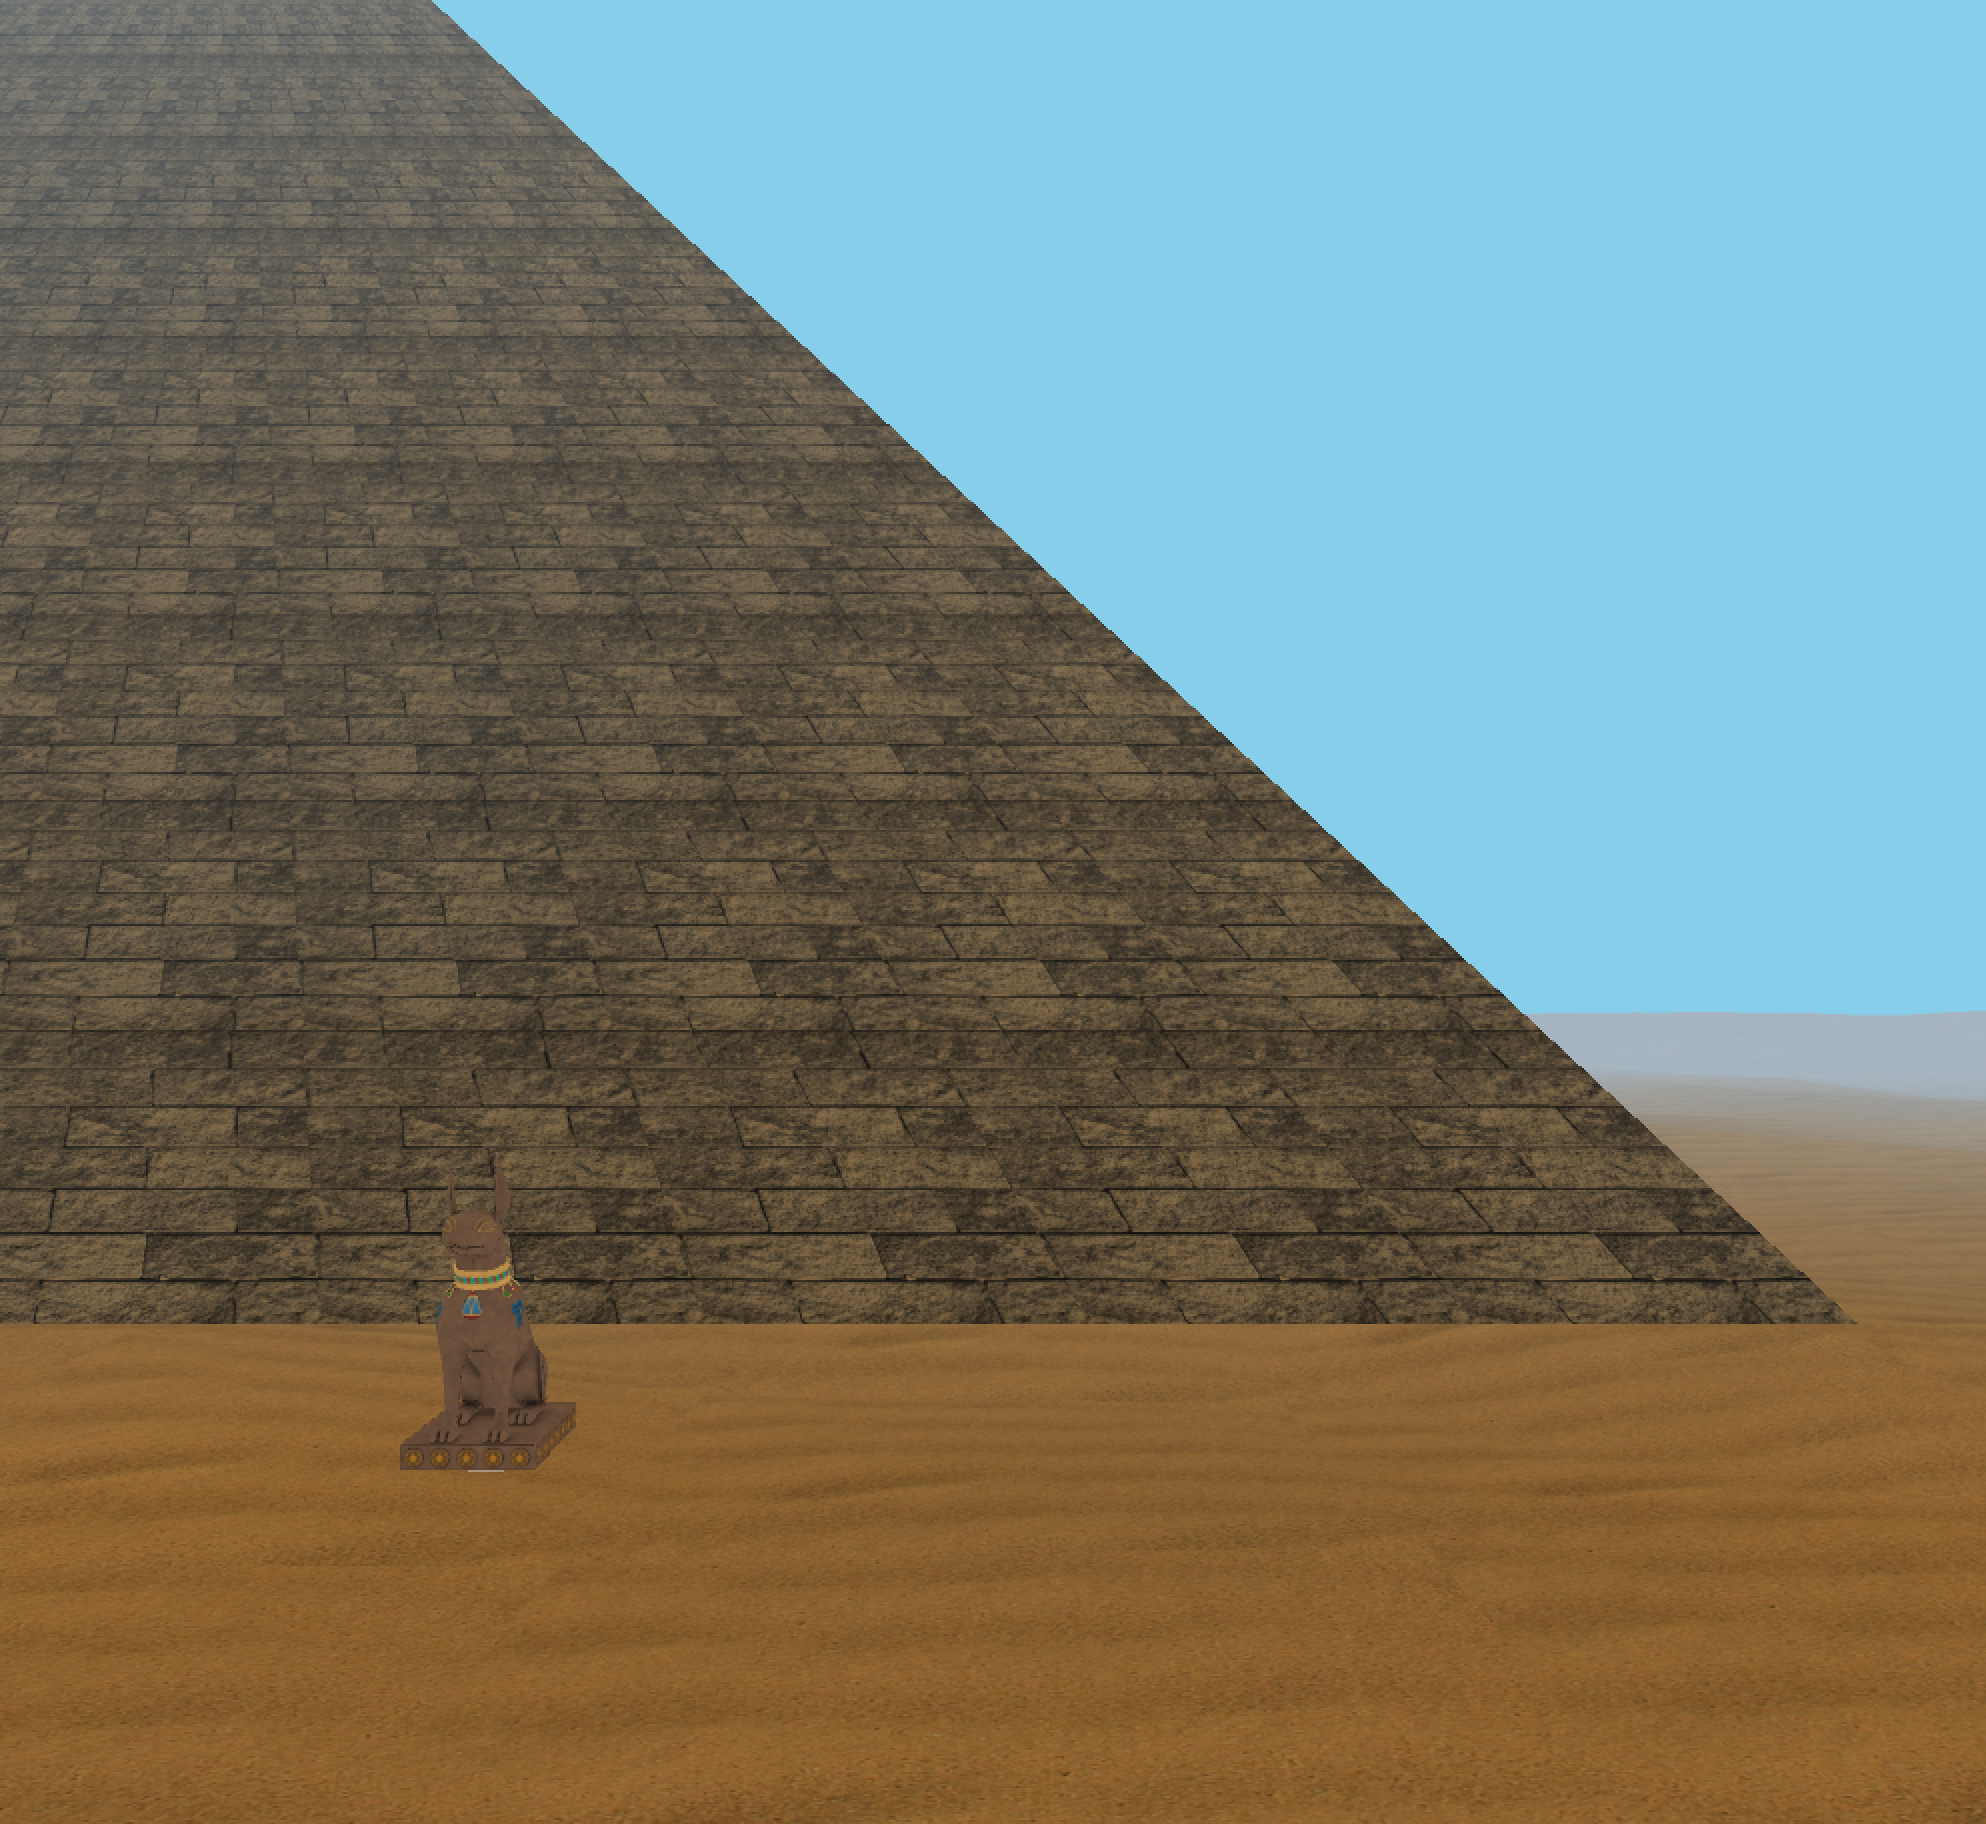
\includegraphics[width=0.8\textwidth]{figures/pyramid-close.png}
    \caption{L'entrée dans la pyramide}
\end{figure}

Dès l’entrée du joueur dans la pyramide, l’interface graphique subit une
modification significative : une mini-carte apparaît, indiquant avec précision
la position actuelle du joueur au sein du labyrinthe ainsi que les trajets déjà
explorés. Initialement, l'ensemble du labyrinthe demeure inconnu, se révélant
au fur et à mesure de l'exploration. De plus, l’interface permet au joueur de
connaître précisément le niveau où il se situe.
\begin{figure}[H]
    \centering
    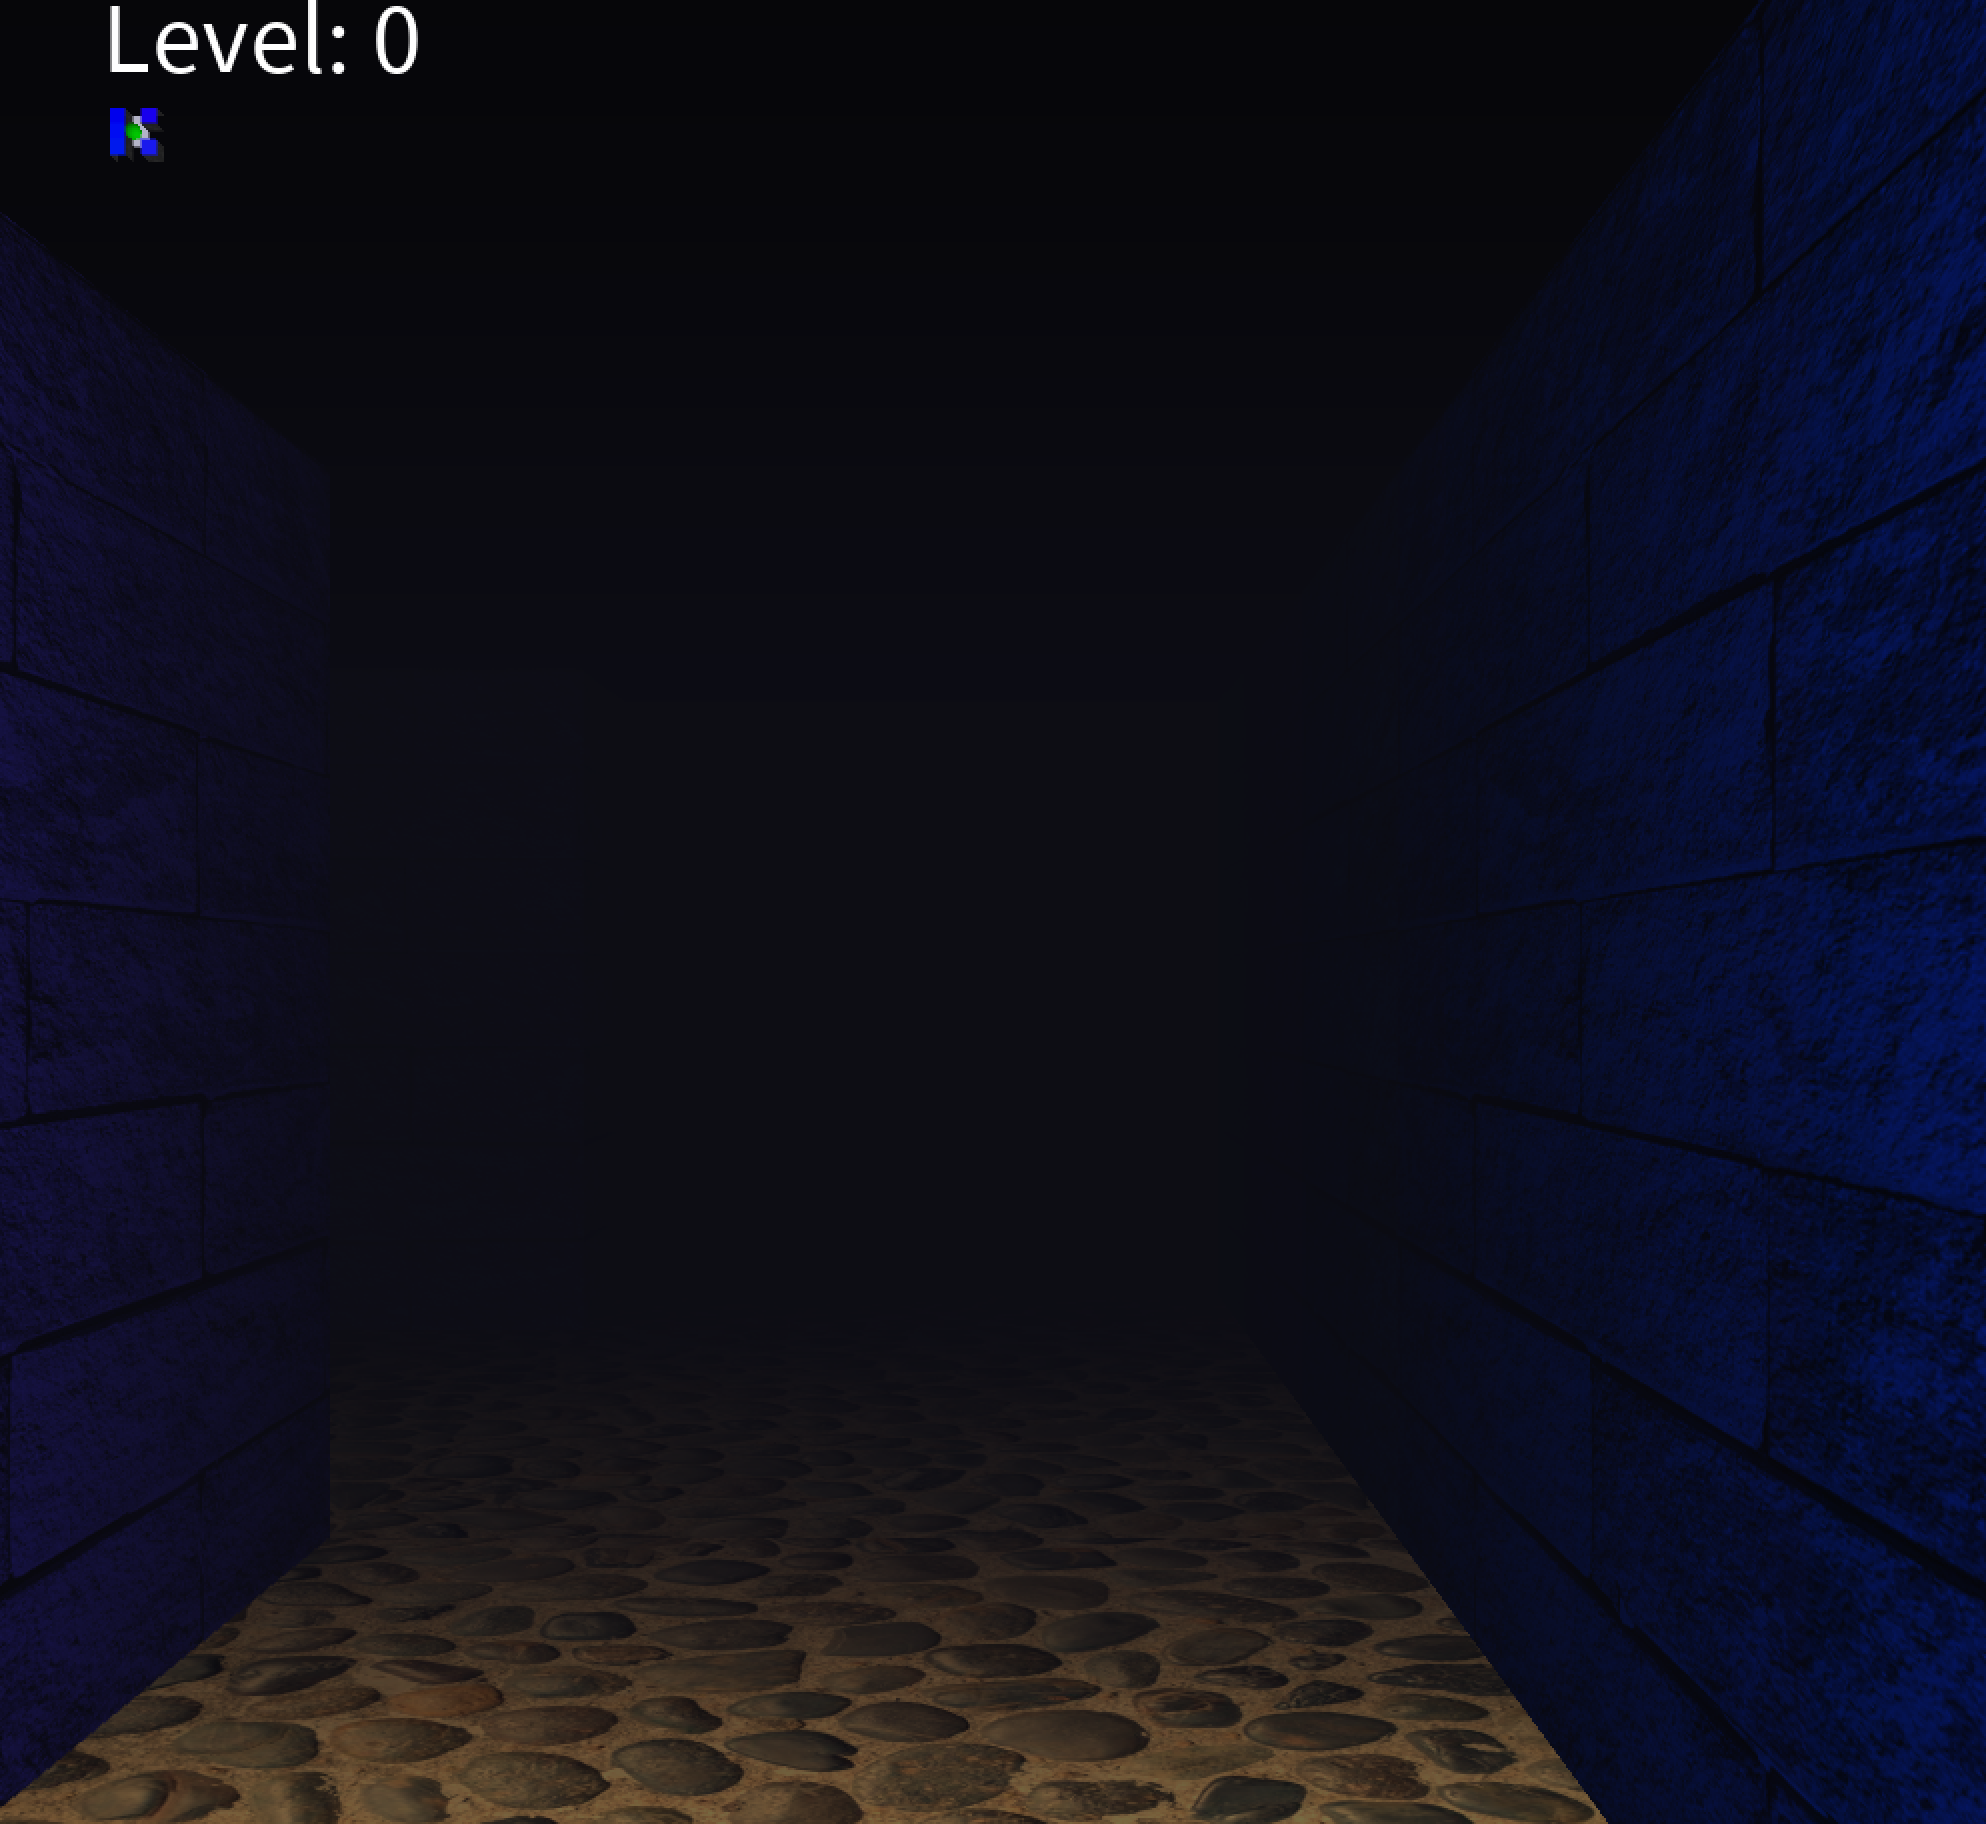
\includegraphics[width=0.8\textwidth]{figures/beg-lab.png}
    \caption{Le début de la labyrinthe}
\end{figure}

Le joueur est rapidement confronté à la momie errant dans le labyrinthe.
Celle-ci est caractérisée par des particules de sable qui s’échappent
continuellement et demeurent temporairement visibles au sol. Ce mécanisme
fournit une indication précieuse quant à sa localisation. Toutefois, toute
interaction directe avec la momie entraîne immédiatement l’affichage du message
« YOU DIED » et la réinitialisation de la position du joueur au début du
labyrinthe, soit au niveau zéro.
\begin{figure}[H]
    \centering
    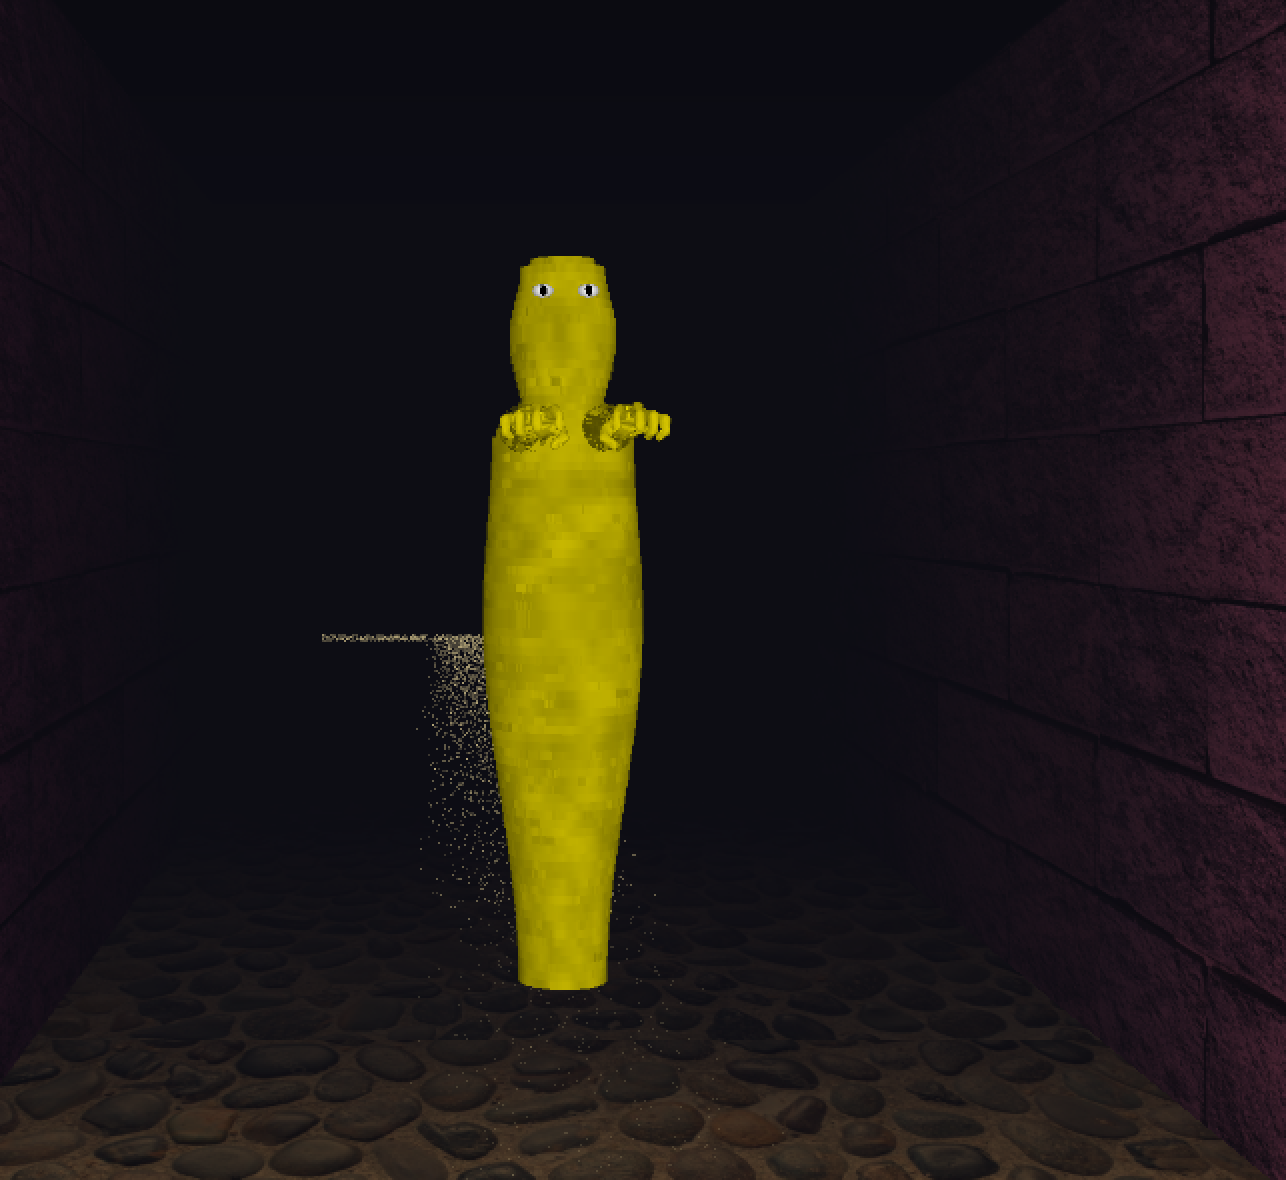
\includegraphics[width=0.8\textwidth]{figures/mummy.png}
    \caption{La momie}
\end{figure}

\begin{figure}[H]
    \centering
    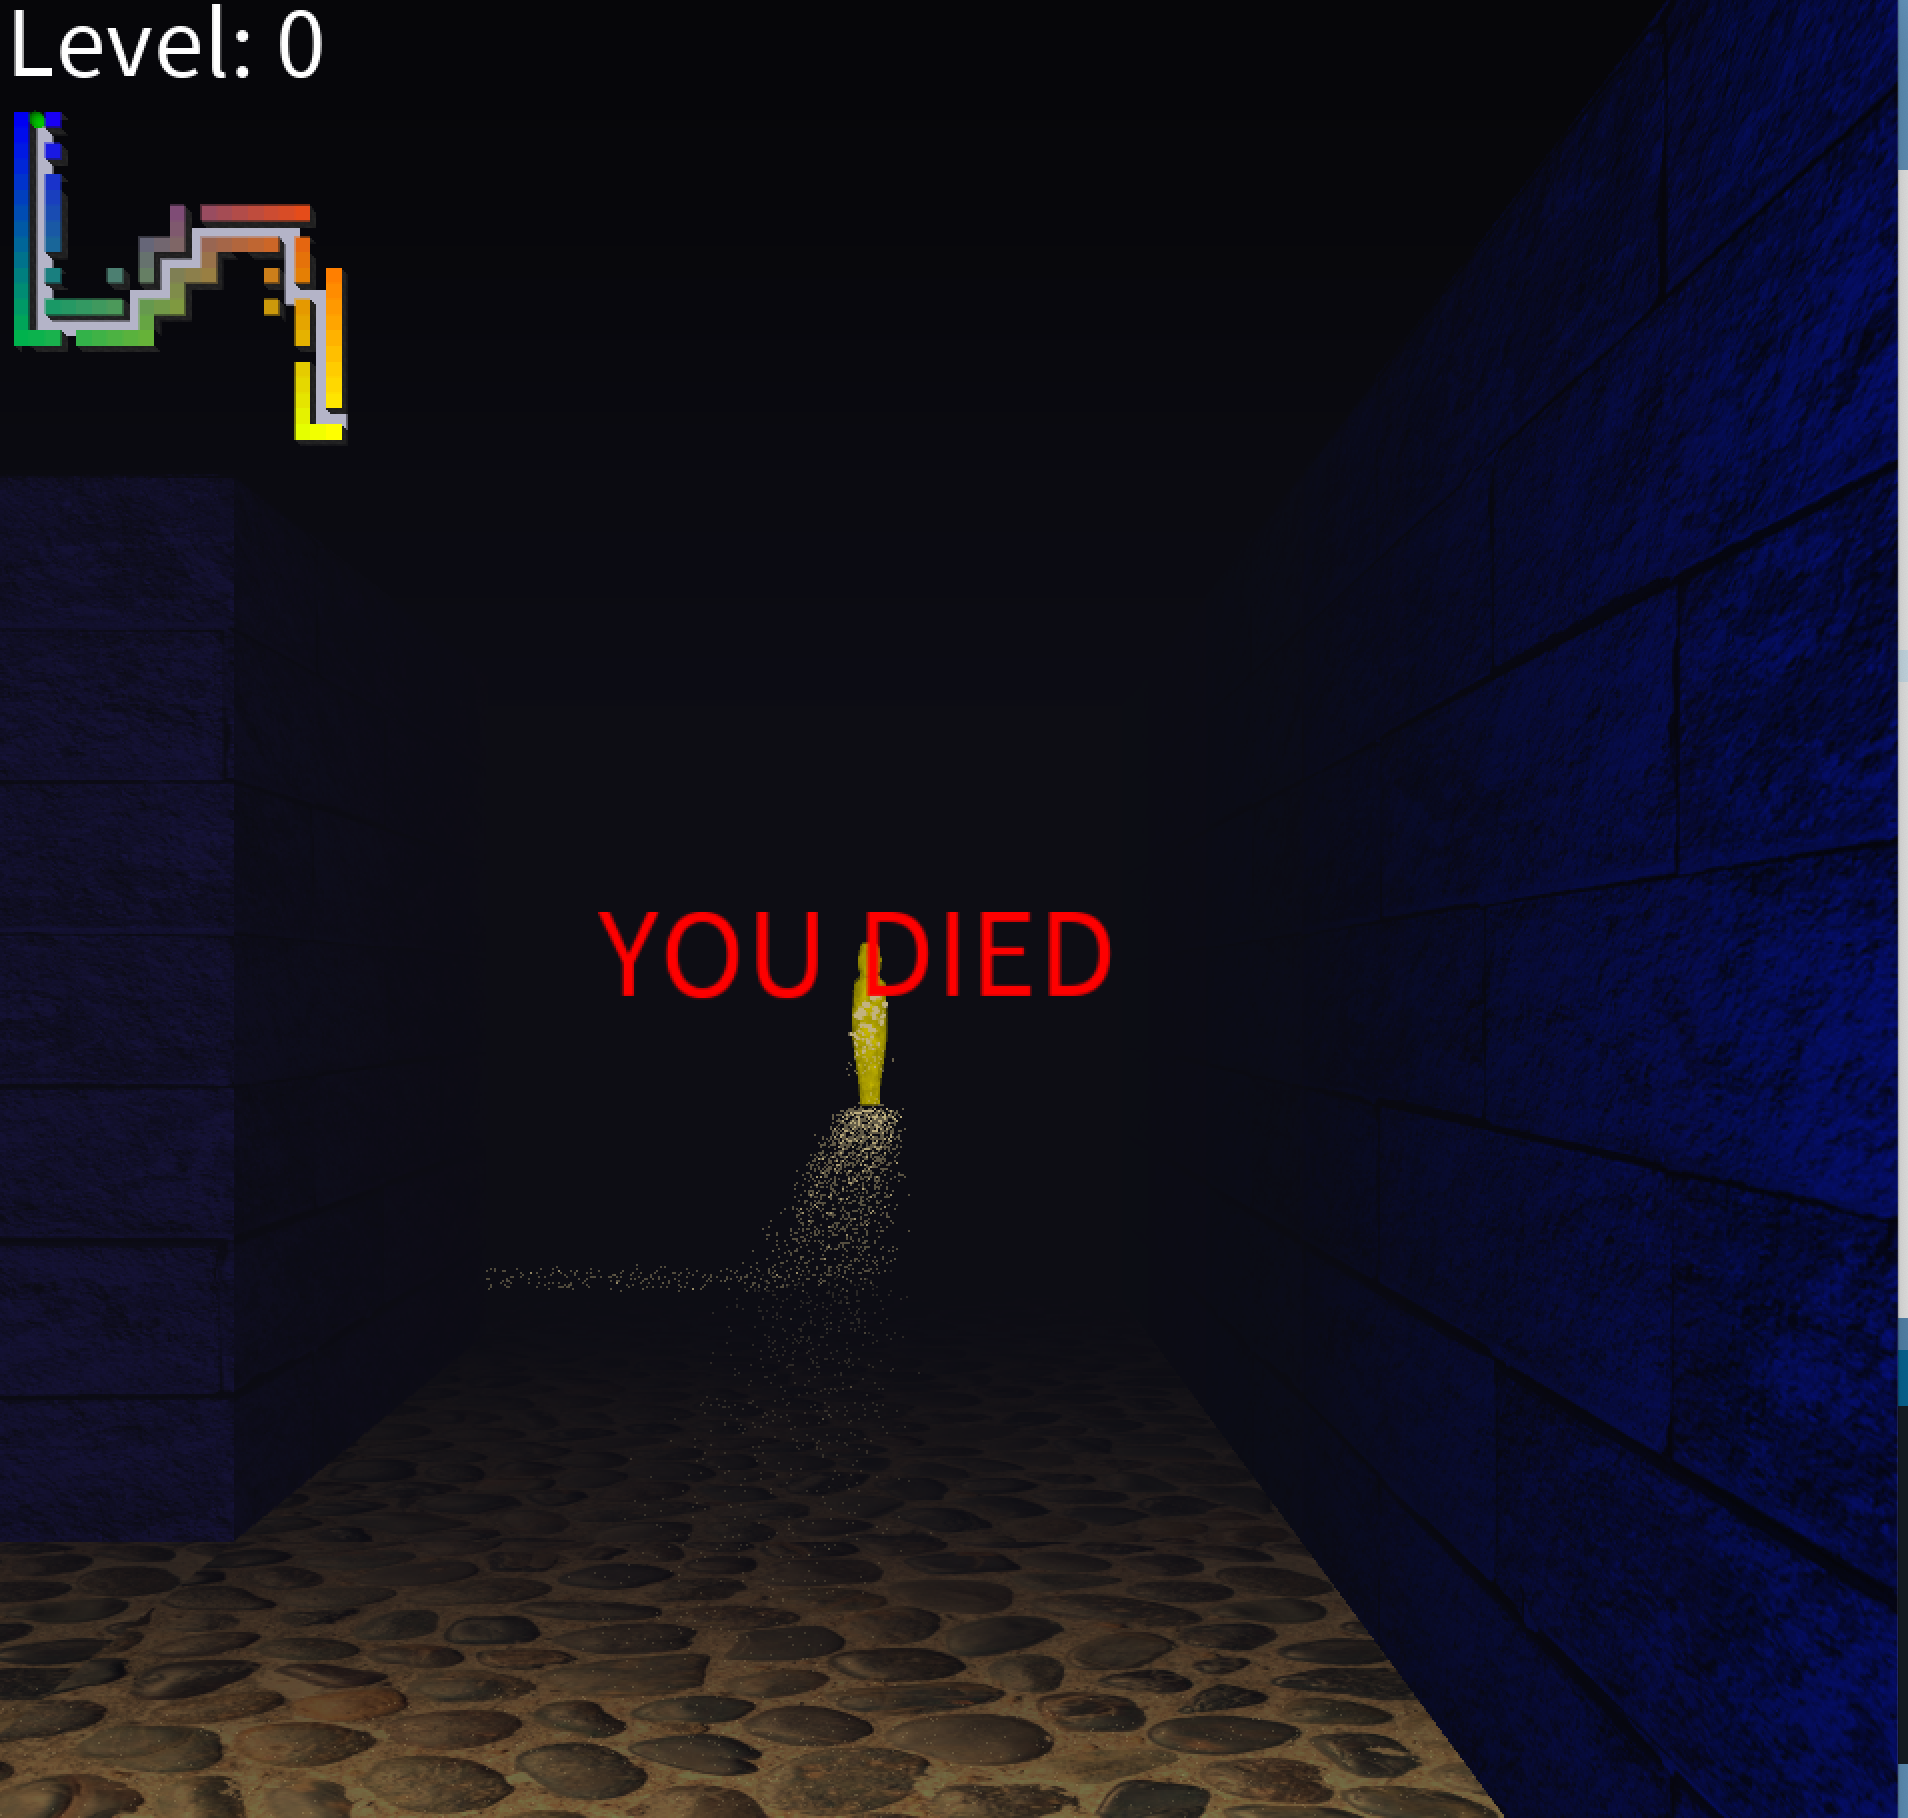
\includegraphics[width=0.8\textwidth]{figures/you-died.png}
    \caption{YOU DIED screen}
\end{figure}

Chaque niveau du labyrinthe, hormis le dernier, est occupé par des momies
semblables. Lorsqu’une sortie est localisée par le joueur, des escaliers
apparaissent, lui permettant ainsi soit de progresser vers le niveau supérieur,
soit de revenir au niveau précédent. L'objectif principal est de naviguer à
travers les différents niveaux du labyrinthe pour atteindre la sortie finale,
tout en évitant les rencontres fatales avec les momies gardiennes.
\begin{figure}[H]
    \centering
    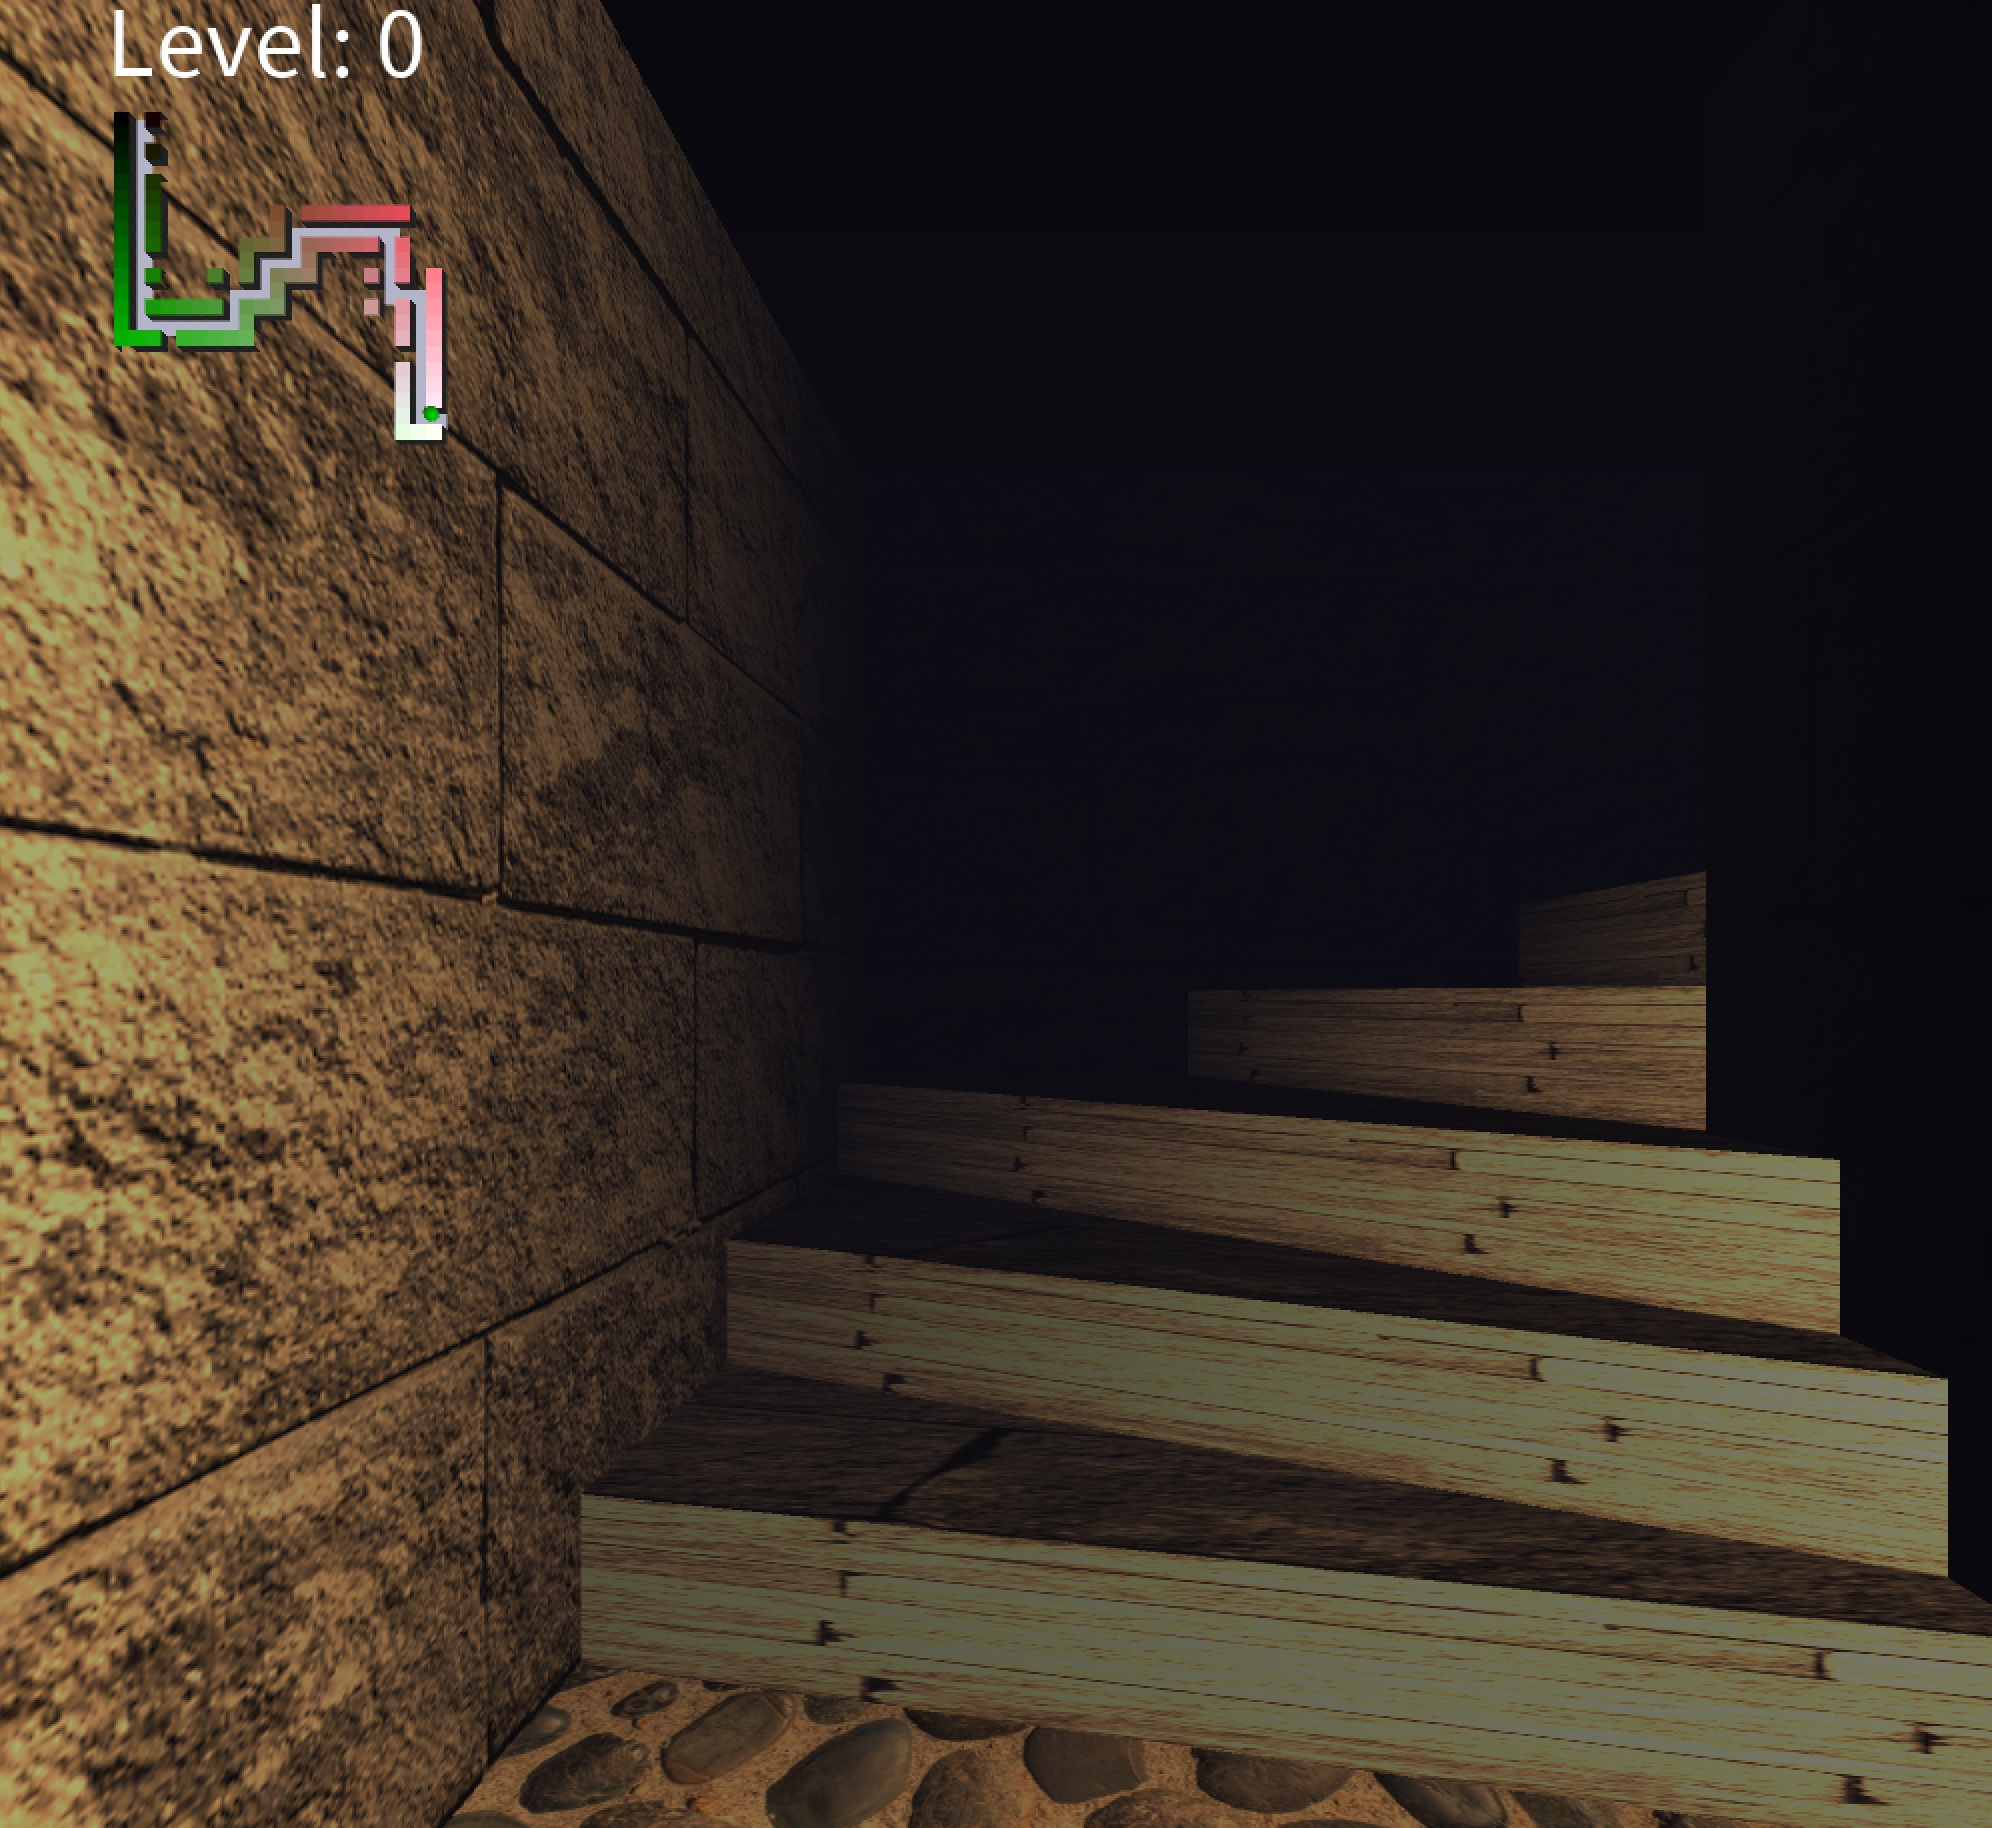
\includegraphics[width=0.8\textwidth]{figures/stairs.png}
    \caption{Les éscaliers}
\end{figure}

\begin{figure}[H]
    \centering
    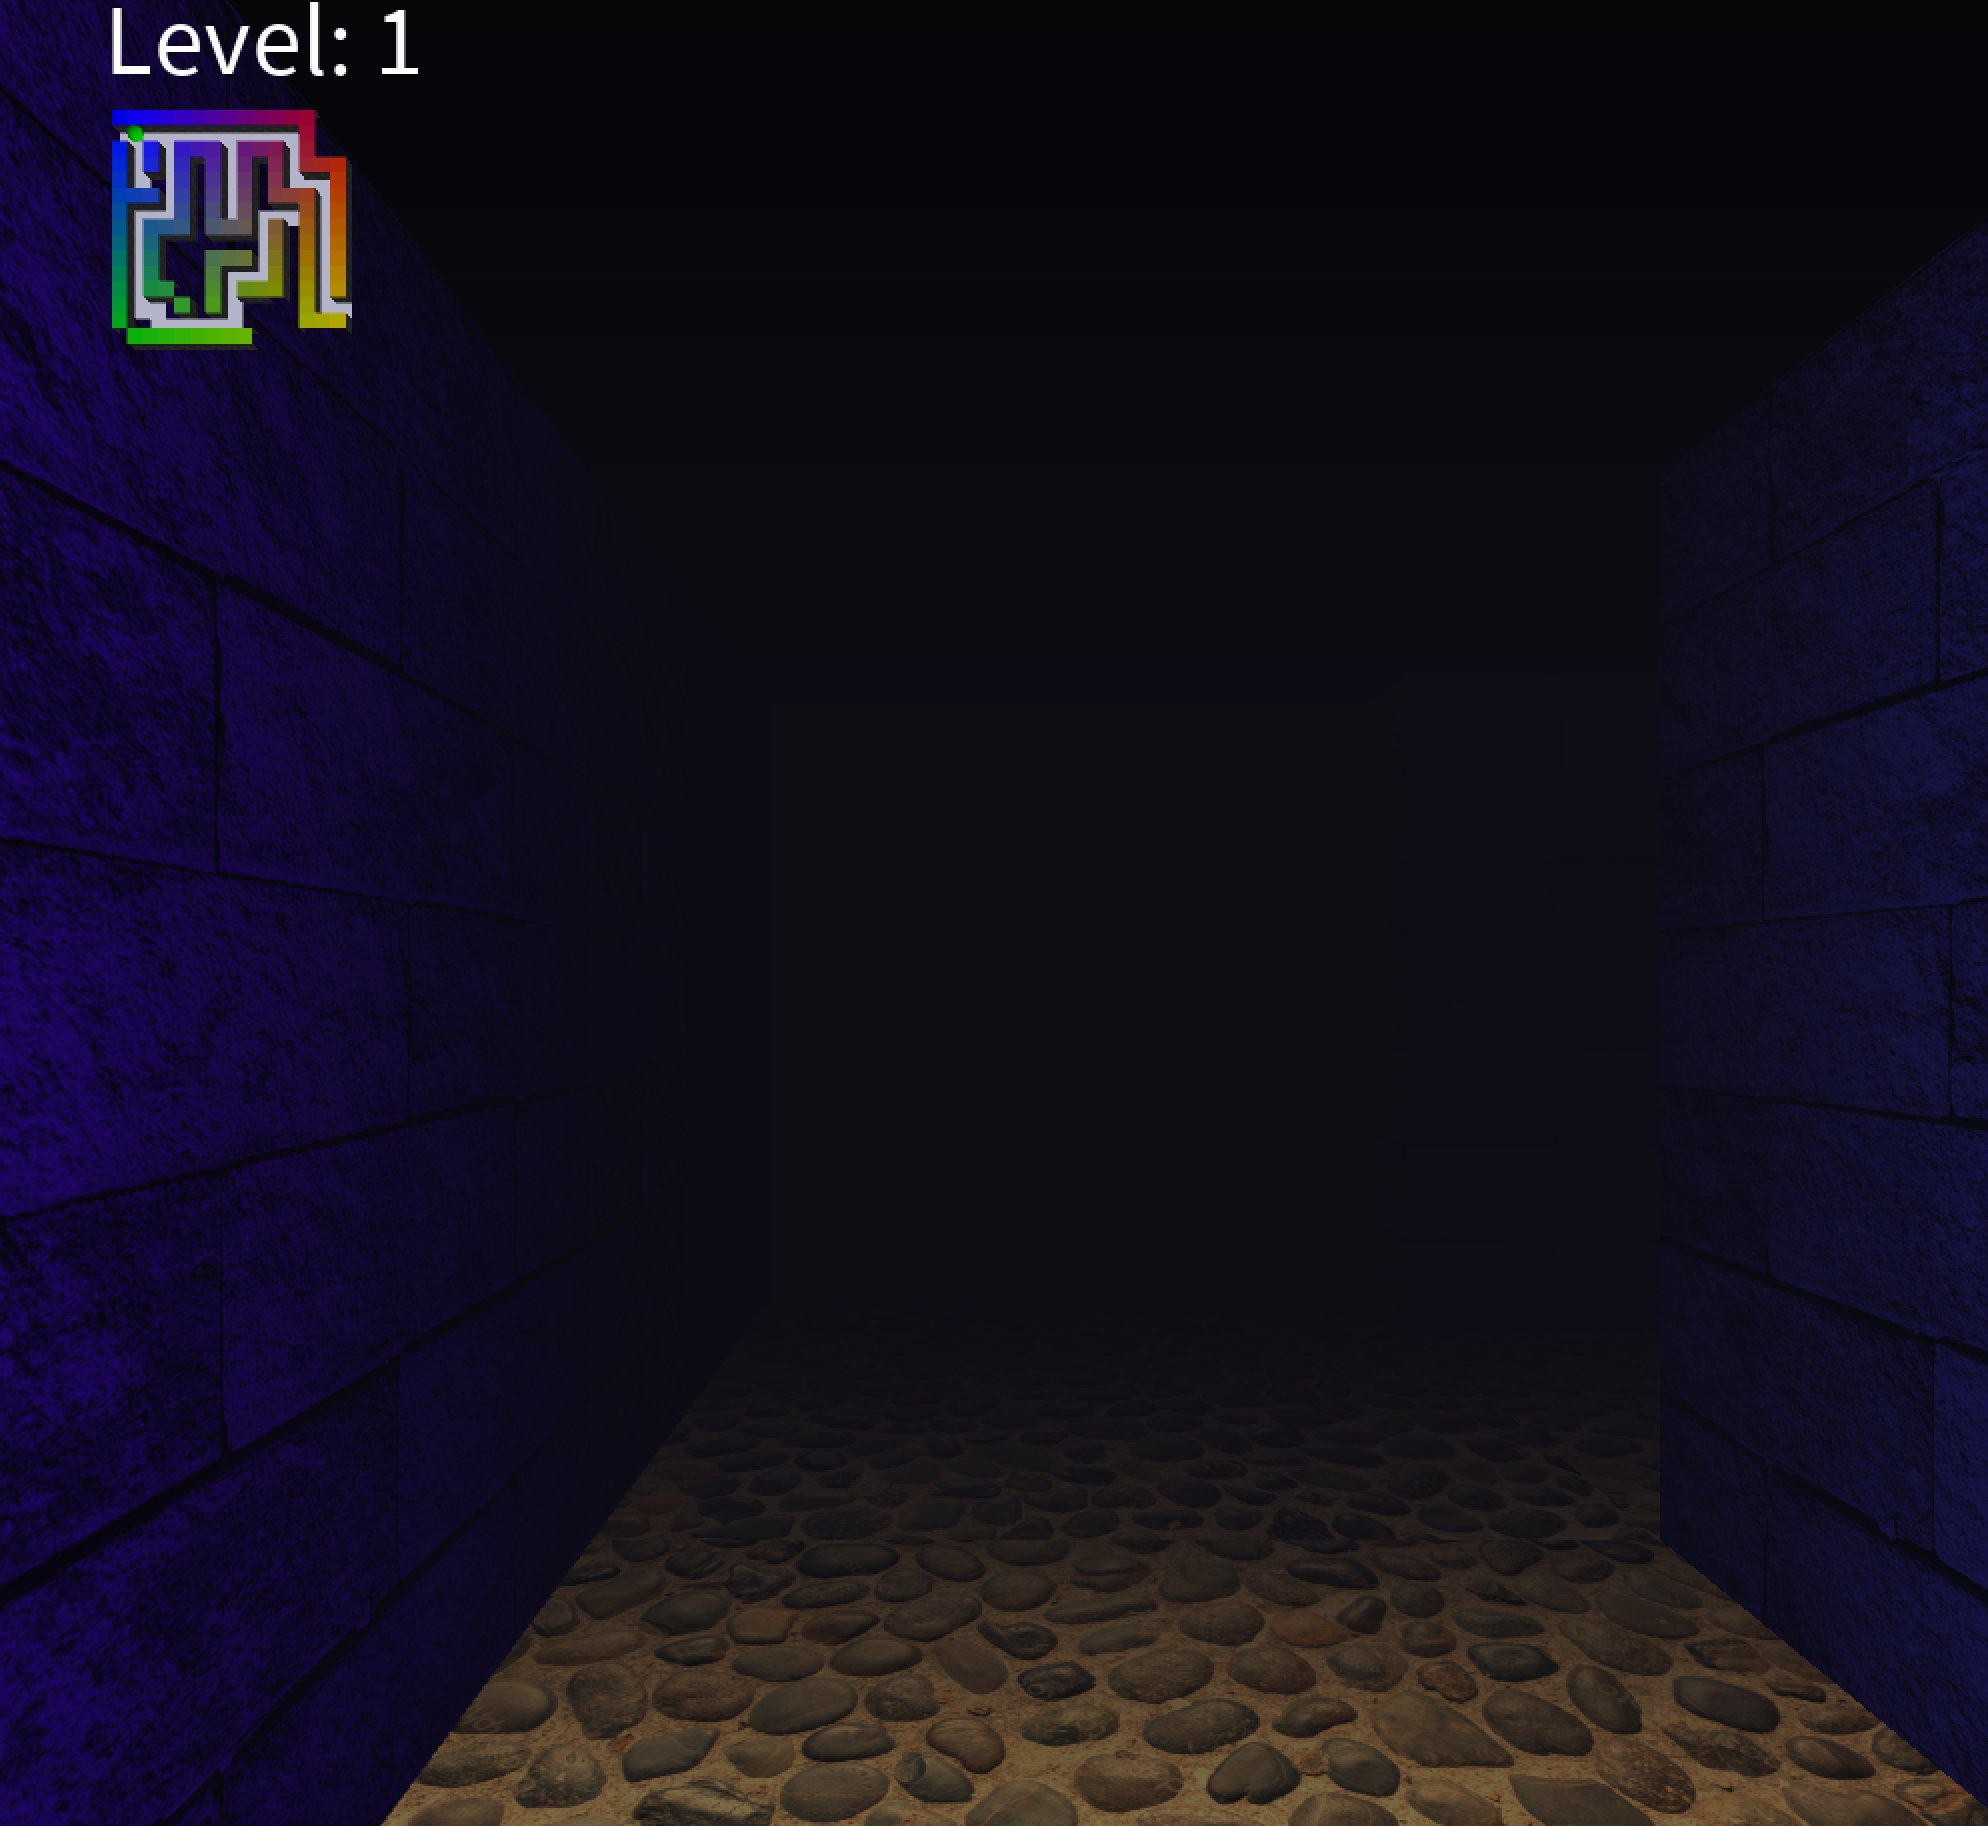
\includegraphics[width=0.8\textwidth]{figures/level1.png}
    \caption{Changement du niveau}
\end{figure}
% -- TODO

\section{Aperçu Technique}
La réalisation de ce projet a mobilisé plusieurs concepts de programmation graphique étudiés en cours, notamment le rendu 3D, la gestion de la caméra, l'application de textures, l'éclairage, les shaders et les systèmes de particules. L'environnement de développement utilisé est Processing et GLSL pour les shaders.

\subsection{Rendu de la Scène Principale (Extérieur)}
La scène extérieure constitue le point de départ du joueur et vise à établir l'atmosphère du jeu.

La pyramide n'est pas un simple modèle 3D mais est construite de manière procédurale dans la fonction drawSteppedPyramid. Elle est composée de plusieurs niveaux. La taille de chaque niveau est calculée par interpolation linéaire \textit{lerp} entre la taille de la base \textit{baseSize} et celle du sommet \textit{topSize} grâce à la fonction \textit{levelSize}. Chaque niveau est dessiné comme un plateau horizontal \textit{QUADS} et des murs inclinés connectant ce niveau au suivant.

Les murs inclinés de la pyramide sont rendus par la fonction drawTexturedWall. Pour améliorer le réalisme et l'application de la texture \textit{wallTexture}, chaque mur est subdivisé horizontalement \textit{wallSubdivisions}. Les coordonnées des sommets de chaque subdivision sont calculées par interpolation linéaire \textit{PVector.lerp} entre les coins du mur complet. La texture est appliquée à chaque segment \textit{QUADS}, en spécifiant les coordonnées de texture \textit{UV} pour mapper l'image stones.jpg.

Un sommet pointu \textit{drawPyramidApex} est ajouté au-dessus du dernier niveau plat de la pyramide, utilisant une géométrie simple de \textit{TRIANGLES} connectant les coins du dernier plateau à un point central élevé.

Le sol \textit{drawDesertFloor} n'est pas plat. Il utilise le bruit de Perlin \textit{noise(}) pour générer des variations de hauteur \textit{noiseHeight} sur une grille de \textit{QUADS}. Cela crée un effet de dunes subtil et irrégulier. La texture sandTexture est appliquée et répétée sur la surface pour simuler le sable.

Un modèle 3D externe représentant une statue d'Anubis \textit{cat.obj} est chargé \textit{loadShape} et positionné dans la scène \textit{shape(cat}). Cela démontre l'intégration d'assets externes.

Shaders Extérieurs (\textit{pyramid\_frag.glsl}, \textit{pyramid\_vert.glsl}) : Lorsque les shaders sont activés \textit{shadersEnabled}, le rendu de la scène extérieure est géré par des shaders \textit{GLSL} personnalisés.

Le vertex shader \textit{\textit{pyramid\_vert.glsl}} transforme les positions des sommets \textit{vertex} dans l'espace de vue et de projection. Il transmet également la normale \textit{normal}, la couleur \textit{color}, les coordonnées de texture \textit{texCoord} et la position dans le monde \textit{vertWorldPos} au fragment shader.

Le fragment shader \textit{\textit{pyramid\_frag.glsl}} calcule la couleur finale de chaque pixel. Il applique la texture \textit{texture2D} et calcule l'éclairage en utilisant un modèle simple : une lumière directionnelle simulant le soleil \textit{sunDirection} avec une composante diffuse (dot(normal, sunDir)) et une lumière ambiante. Une légère distorsion visuelle basée sur la position et le temps (sin(vertWorldPos.x * ... + time * ...)), ainsi qu'un effet de brouillard basé sur la distance (mix(skyColor, litColor, fogFactor)) sont ajoutés pour l'atmosphère. La saturation est légèrement augmentée (mix(grayScale, litColor.rgb, 1.2)).

\subsection{Labyrinthe Intérieur}
Le labyrinthe est défini par des tableaux
de caractères 2D pour chaque niveau (\textit{labyrinthe[][][]} dans
\textit{set\_labyrinths}). La fonction \textit{drawLabyrinth} (et sa variante
\textit{drawLabyrinthWithoutSpheres}) parcourt ce tableau. Si une cellule
contient "\#", un mur est dessiné. Si elle contient " ", un sol et un plafond
sont dessinés. Les murs ne sont dessinés que sur les faces exposées (en
vérifiant les cellules adjacentes) pour optimiser le rendu. Les murs, sols et
plafonds sont dessinés comme des \textit{QUADS} texturés (\textit{stone} et \textit{floor\_texture}). La
taille de chaque cellule est définie par \textit{cellSize}.

La source de lumière principale est une torche virtuelle portée par le joueur. Sa position (\textit{playerWorldX}, \textit{playerWorldY}, \textit{playerWorldZ}) est calculée dans le sketch principal et envoyée au shader (\textit{torchPosWorld} → \textit{torchPosView}). Le fragment shader (\textit{labyrinth\_frag.glsl}) implémente cette torche comme une source de lumière ponctuelle. La fonction \textit{calculatePointLight} détermine l'intensité lumineuse en fonction de la distance (\textit{distSqr}, \textit{radiusSqr}) et de l'angle par rapport à la surface (\textit{NdotL}). L'intensité (\textit{torchBrightness}) et la couleur (\textit{torchColor}) sont paramétrables. Un effet de scintillement (\textit{flicker}) est ajouté en modulant la luminosité avec une fonction sinus basée sur le temps (\textit{time}).

Des sphères colorées lumineuses sont placées à des endroits spécifiques (culs-de-sac, coins) pour guider subtilement le joueur et ajouter de l'intérêt visuel. La fonction \textit{identifyBallLights} parcourt la carte, détecte ces emplacements spécifiques et stocke les positions (\textit{ballLightWorldPos}) et couleurs (\textit{ballLightColorsForShader}) des lumières trouvées (jusqu'à \textit{MAX\_BALL\_LIGHTS}). Ces informations sont envoyées au shader sous forme de tableaux uniformes (\textit{ballLightViewPositions}, \textit{ballLightColors}). Le fragment shader itère sur ces lumières et additionne leur contribution (\textit{totalBallLightContribution}), en utilisant la même fonction \textit{calculatePointLight}. La géométrie des sphères elles-mêmes est dessinée séparément dans \textit{drawColoredBalls} après le rendu principal avec le shader.

Un brouillard dense (\textit{fogColor}) est appliqué pour limiter la visibilité et renforcer l'atmosphère oppressante. Le facteur de brouillard (\textit{fogFactor}) est calculé dans le vertex shader en fonction de la distance de la caméra (\textit{vertViewPos.z}) et appliqué dans le fragment shader (\textit{mix(fogColor.rgb, finalLitColor, fogFactor)}).

Une très faible lumière ambiante (\textit{minAmbient}) est ajoutée dans le shader pour s'assurer que les zones non éclairées ne sont pas complètement noires.

Des modèles d'escaliers (\textit{drawStairs}, \textit{drawDownStairs} dans \textit{stairs.pde}) sont placés aux positions de sortie (\textit{endPosX}, \textit{endPosY}) et d'entrée (\textit{descendPosX}, \textit{descendPosY} ou \textit{startPosX}, \textit{startPosY} selon le niveau) de chaque étage. La fonction \textit{keyPressed} détecte si le joueur atteint l'une de ces cases en avançant. Si c'est le cas, la variable \textit{current\_lab\_level} est modifiée, et les coordonnées du joueur (\textit{posX}, \textit{posY}) sont réinitialisées aux coordonnées de départ du nouveau niveau, simulant ainsi un "téléportage" entre les étages. Une courte animation de caméra (\textit{anim}, \textit{state = turn\_repl.going\_forward}) accompagne ce changement.

\subsection{Momie}

L'antagoniste principal du jeu est la momie.

La momie (\textit{mummy.pde}) est un \textit{PShape} complexe construit de manière procédurale. Le corps (\textit{createBodyShape}) est formé d'une série d'anneaux (\textit{QUAD\_STRIP}) dont le rayon (\textit{R}) varie le long de l'axe vertical (interpolé avec \textit{smoothstep}) pour créer la silhouette. Une légère variation de couleur basée sur le bruit (\textit{noise()}) est appliquée à chaque anneau pour simuler des bandages irréguliers. Les yeux (\textit{createEyeShape}) sont des sphères simples. Les bras (\textit{createHandShape}) sont également des séries d'anneaux. Les poignets (\textit{createWristShape}) sont des modèles .obj chargés (\textit{hand1.obj}, \textit{hand2.obj}). L'ensemble est assemblé et mis à l'échelle dans \textit{createMummy}.

La momie se déplace de manière aléatoire dans le labyrinthe en respectant des règles déterminées. Dans un premier temps, elle progresse toujours en ligne droite. Si un mur se trouve directement devant elle et qu’aucune autre direction n’est accessible, elle effectue un virage à 180° pour rebrousser chemin. Dans le cas où plusieurs options s’offrent à elle, la direction est choisie aléatoirement. Par ailleurs, lorsqu’elle se trouve dans un carrefour --- c’est-à-dire qu’il n’y a pas de mur devant elle, mais que des possibilités de tourner existent ---, la momie continue tout droit avec une probabilité de 50 % (valeur susceptible d’être ajustée) ou, alternativement, opte pour une autre direction de façon aléatoire.

Pour indiquer la présence de la momie, un système de particules de sable est implémenté. La classe \textit{SandParticle} définit une particule avec une position, une vélocité, une durée de vie et un état. Dans \textit{drawMummy}, de nouvelles particules sont générées (\textit{new SandParticle}) près de la position de la momie avec une vélocité initiale aléatoire. La fonction \textit{update()} de chaque particule applique une force de gravité, met à jour la position, et détecte si la particule a touché le sol. Une fois au sol, la particule reste visible pendant un certain délai (\textit{landedDelay}) avant de disparaître (son alpha diminue avec \textit{age}). Les particules sont dessinées comme des points avec une taille et une transparence variables. Ce choix d'affichage en points, plutôt qu'en utilisant des sphères, a été adopté afin d'optimiser les performances, car l'utilisation de sphères entraînait des ralentissements significatifs dans le rendu du système de particules.

Dans la boucle \textit{draw} principale, une simple vérification de collision est effectuée : si les coordonnées de grille du joueur sont identiques à celles de la momie (\textit{mummyInitX}, \textit{mummyInitY}), le joueur meurt (\textit{playerDead = true}). Un message "YOU DIED" s'affiche (\textit{drawGameOver}), et après un court délai, le joueur est réinitialisé au début du labyrinthe (\textit{current\_lab\_level = 0}, \textit{posX = 1}, \textit{posY = 0}).

\subsection{Organisation du Code}

Le projet est structuré en plusieurs fichiers \texttt{.pde} pour une meilleure organisation :

\begin{itemize} \item \textit{sketch\_250314a.pde} : Fichier principal contenant \textit{setup()}, \textit{draw()}, \textit{keyPressed()}, les variables globales, la gestion de l'état du jeu et la logique de caméra. \item \textit{pyramid.pde} : Contient les fonctions spécifiques au rendu de la scène extérieure (pyramide, désert). \item \textit{labyrinth.pde} : Gère la définition, le rendu du labyrinthe, la mini-carte, l'indicateur de niveau et la logique des lumières sphériques. \item \textit{mummy.pde} : Contient toute la logique et le rendu de la momie, y compris le système de particules de sable. \item \textit{stairs.pde} : Fonctions pour dessiner les modèles d'escaliers. \end{itemize}

\textit{data/} : Dossier contenant les assets : textures (\texttt{.jpg}), modèles 3D (\texttt{.obj}) et les fichiers de shaders (\texttt{.glsl}).

Cette organisation permet de séparer les différentes fonctionnalités du jeu, rendant le code plus facile à lire, à comprendre et à maintenir.

Pour la gestion de version, nous avons créé un dépôt sur GitHub, ce qui nous permet de partager nos avancées entre nous et de faciliter le suivi et le contrôle des modifications.

\section{Conclusion}
Ce projet a été une excellente opportunité d'appliquer les concepts de programmation graphique 3D appris en cours dans un contexte ludique. La création de la pyramide procédurale, l'implémentation de l'éclairage dynamique avec des shaders GLSL (notamment la gestion de plusieurs sources lumineuses et les effets comme le scintillement et le brouillard), et le développement de déplacement simple, mais efficace de la momie ont été des aspects particulièrement formateurs.

Les défis rencontrés incluaient le débogage des shaders GLSL, en particulier le passage correct des données (comme les positions des lumières sphériques) du code Processing vers les shaders, ainsi que l'ajustement des paramètres d'éclairage et de brouillard pour obtenir l'atmosphère souhaitée. La logique de déplacement de la momie a également nécessité plusieurs itérations pour obtenir un comportement crédible. Par ailleurs, des problèmes d’optimisation ont été abordés tant pour les shaders que pour les objets du jeu. Ces optimisations ont permis de réduire significativement la charge de calcul et d'améliorer ainsi la réactivité et la fluidité du rendu graphique global.

Pistes d'Amélioration Futures :

\begin{itemize}
    \item 
        Mouvement de la Momie : Rendre la momie plus intelligente, capable de "chasser" le joueur au lieu de se déplacer aléatoirement.
    \item
        Variété des Niveaux : Ajouter plus de diversité dans la structure des niveaux, peut-être avec des pièges ou des énigmes simples.
    \item
        Optimisation : Analyser les performances et optimiser le rendu, notamment si des niveaux plus grands ou plus d'ennemis étaient ajoutés.
    \item
        Interactions : Ajouter plus d'éléments interactifs dans l'environnement.
    \item
        En conclusion, ce projet a permis de consolider ma compréhension des techniques de rendu 3D temps réel et de la programmation de shaders, tout en offrant une expérience de développement de jeu stimulante..
\end{itemize}



\end{document}
